\documentclass[11pt]{amsart}
\usepackage[numbers]{natbib}

\usepackage{microtype}
\usepackage{float}
\usepackage[margin=1in]{geometry}
\usepackage{graphicx}
\usepackage{url}

\usepackage{amsmath, amssymb, amsthm}
\usepackage[version=4]{mhchem}
\usepackage{siunitx}
\usepackage{longtable,tabularx}
\usepackage{mdframed}
\setlength\LTleft{0pt} 

\newtheorem{theorem}{Theorem}[section]      % numbering within sections
\newtheorem{lemma}[theorem]{Lemma}         % same counter as theorem
\newtheorem{proposition}[theorem]{Proposition}
\newtheorem{corollary}[theorem]{Corollary}

\theoremstyle{definition}                  % for non-italic style
\newtheorem{definition}[theorem]{Definition}
\newtheorem{example}[theorem]{Example}

\theoremstyle{remark}                      % for remarks
\newtheorem{remark}[theorem]{Remark}

\usepackage{hyperref}

\newmdtheoremenv[
    linecolor=black,
    linewidth=1pt,
    roundcorner=5pt,
]{boxedtheorem}[theorem]{Theorem}


\title{Early Topics and Examples in Optimal Transport}

\author{Asher Christian}


\begin{document}

\maketitle

\begin{abstract}
    The goal of this text is to develop the foundations of optimal transport using only the tools
    of measure theory taught in Math 245A and some basic probability theory. 
    I establish necessary results from measure theory, including Prokhorov's theorem and properties of weak convergence, to provide
    a self-contained proof of the existence of optimal transport plans.
\end{abstract}

\section{Introduction}
Optimal transport seeks to provide the most efficient way to move mass from one distribution to another while minimizing a specific cost.
The theory has applications in numerous fields, from machine learning to economics.
The concept of optimal transport was first proposed by French mathematician Gaspard Monge in 1781 \citep{monge1781ot}. Later, during World War II,
the Soviet mathematician Leonid Kantorovich greatly advanced the topic by proving that solving the problem of finding an optimal transport plan is equivalent under certain conditions
to maximizing a dual variable \citep{kantorovich1942english}.
I will mainly be following the works of C\'edric Villani \citep{villani2008ot} in establishing the existence of solutions to the problem as well as providing examples.

\section{Notation}

{\renewcommand\arraystretch{1.0}
\noindent\begin{longtable}{@{}l @{\quad-\quad} l@{}}
    $(\mathcal{X}, \mathcal{B})$ & A measurable space $\mathcal{X}$ and the set of measurable sets $ \mathcal{B} \subset 2^{ \mathcal{X}}$. \\
    $(\mathcal{X}, \mathcal{B}, \mu)$ & A measure space with measure $\mu$. \\
    $(\mathcal{X}, \mu)$ & $(\mathcal{X}, \mathcal{B},\mu)$ where $ \mathcal{B}$ are the Borel measurable sets under the condition that $\mathcal{X}$ has a topology.\\
    $P( \mathcal{X})$ & The set of all Borel probability measures on $\mathcal{X}$.\\
    $X_*( \mathbb{P})$ & The pushforward measure induced by $X: (\Omega, \mathcal{F}, \mathbb{P}) \rightarrow ( \mathcal{X})$ measurable.\\
                       & $X_*( \mathbb{P})(A) = \mathbb{P}(X^{-1}(A))$\\
    $\sigma(\mathcal{P})$ & The $\sigma$-algebra generated by $\mathcal{P}$ whenever $\mathcal{P} \subset 2^{\Omega}$ is a collection of sets.\\
    $ \mathbb{R}^{+}$ & $ \mathbb{R} \cap [0,\infty)$ the nonnegative real numbers.\\
    $\langle A, B \rangle_F$ & $\sum_{i=1}^{n} \sum_{j=1}^{m} A_{i,j} B_{i,j}$ the Frobenius inner product of two $n \times m$ real matrices $A,B$.
\end{longtable}}

\section{Introducing the Problem}
Before we state the problem, we must first introduce a basic notion of couplings at the level of measures.
\begin{definition}[Couplings]
    Let $(\mathcal{X},\mu), (\mathcal{Y}, \nu)$ be two probability spaces. The set $\Pi(\mu,\nu)$ is defined to be the set of all Borel probability
    measures $\pi$ on $\mathcal{X} \times \mathcal{Y}$ satisfying  $\pi(A \times \mathcal{Y}) = \mu(A), \pi(\mathcal{X} \times B) = \nu(B)$ for all $A \subset \mathcal{X}, B \subset \mathcal{Y}$ measurable sets.
    That is, $\pi$ admits as marginals the measures $ \mu $ and $\nu$. These measures are referred to as \textbf{couplings}.
\end{definition}
\begin{remark}
The set of couplings is non-empty since one can always construct the independent coupling $\mu \times \nu$ referred to as the product measure as shown in Proposition 1.7.11 of Tao \citep{Tao2011Measure}. The existence
of this measure was proven under the condition that $(\mathcal{X}, \mu)$ and $(\mathcal{Y}, \nu)$ are  $\sigma$-finite measure spaces which they trivially are since $\mu(\mathcal{X}) = \nu(\mathcal{Y}) = 1$.
\end{remark}
\begin{remark}
    The set of couplings is also closed under convex combinations. Formally, if $\pi_1,\dots,\pi_k$ are couplings of $\mu$ and $\nu$, and
     if $\lambda_1, \dots, \lambda_k \ge 0$ satisfy $\sum_{i=1}^{k}\lambda_i = 1$, then
     \[
     \pi := \sum_{i=1}^{k}\lambda_i\pi_i
     \] 
     is a coupling. Indeed, for any Borel set $A \subset \mathcal{X}$,
     \[
     \pi(A \times \mathcal{Y}) = \sum_{i=1}^{k}\lambda_i \pi(A \times \mathcal{Y}) = \sum_{i=1}^{k}\lambda_i \mu(A) = \mu(A)
     \] 
     with a similar result for any $B \in \mathcal{Y}$. Once we have multiple couplings, we can construct infinitely many more by creating convex combinations of our existing couplings.
\end{remark}

\begin{definition}[MKp]\label{def:MKp}
    Fix $( \mathcal{X}, \mu), (\mathcal{Y}, \nu)$ two probability spaces and let $c: \mathcal{X} \times \mathcal{Y} \rightarrow  \mathbb{R} \cup \{+\infty\}$ be a cost function. 
    We say a coupling $\pi_{ot} \in \Pi(\mu,\nu)$ is a solution to the \textbf{Monge-Kantorovich minimization problem} (MKp) if 
\begin{equation}\label{MKp}
    \int_{\mathcal{X} \times \mathcal{Y}}^{}c(x,y)d\pi_{ot}(x,y) = \inf_{\pi \in \Pi(\mu,\nu)} \int_{ \mathcal{X} \times \mathcal{Y}}^{}c(x,y)d\pi(x,y)
\end{equation}
\end{definition}

\section{Examples of Couplings}\label{section:example}
Clearly, many couplings are not optimal.
To keep the first example simple, consider a village living on the real line $\mathcal{X} = \mathcal{Y} = \mathbb{R}$.
The village has three olive trees at positions $3$, $10$, and $15$, which produce a third of a ton of olives each.
The village also has two olive presses at positions $3$ and $12$ which each require half a ton of olives to efficiently
produce olive oil. Mathematically we let $\mu = \frac{1}{3}(\delta_3 + \delta_{10} + \delta_{15})$ $\nu = \frac{1}{2}(\delta_3 + \delta_{12})$ 
where $\delta_x$ is the Dirac measure centered at point $x$. Then, in the absence of a cost function
we can construct the independent coupling $\pi = \mu \times \nu$ as in figure \ref{fig:independent-example}.
\begin{figure}[H]
    \centering
    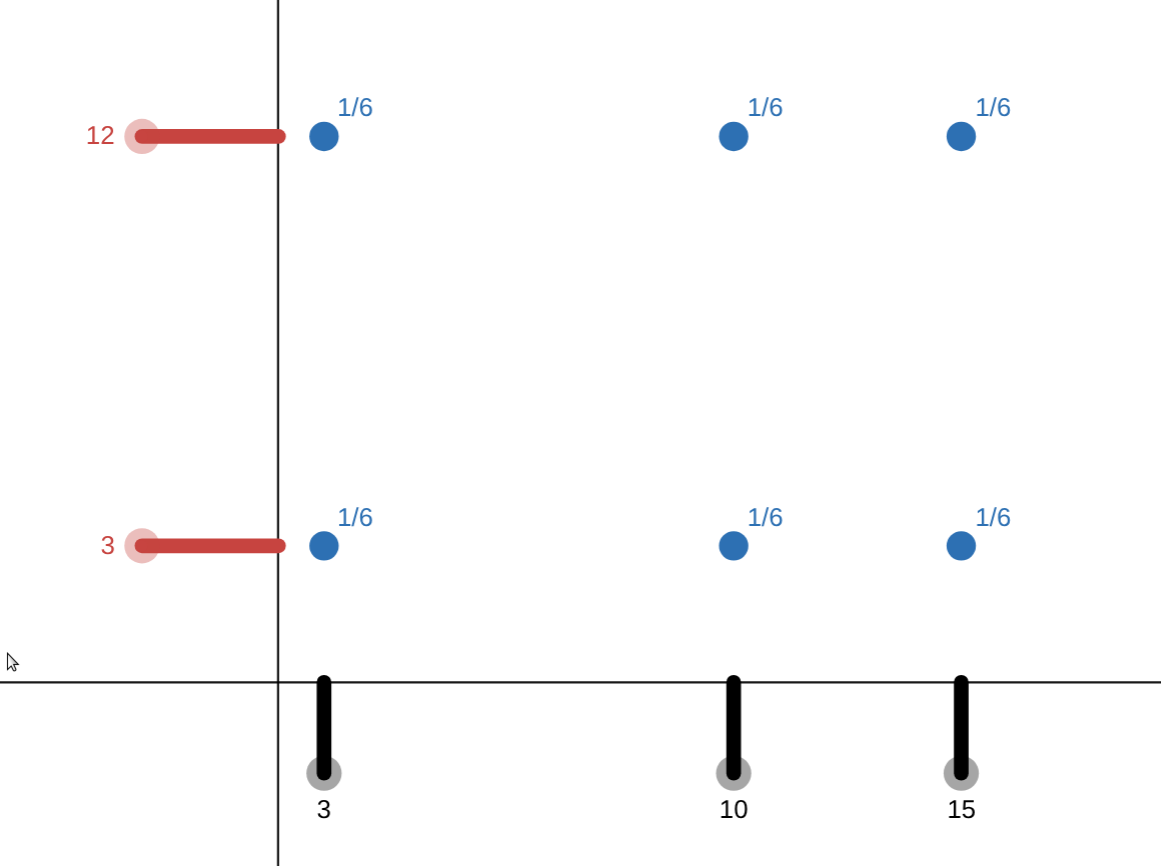
\includegraphics[width=0.5\textwidth]{Picture1.png}
    \caption{Independent coupling between two discrete measures.}
    \label{fig:independent-example}
\end{figure}
Additionally, using the fact that every coupling of sums of Dirac measures is a sum of Dirac measures, we can say
that every coupling is of the form:
\begin{equation}\label{eq:discrete_coupling}
    \pi_{\vec c} = c_1\delta_{3,3} + c_2\delta_{10,3} + c_3\delta_{15,3} + c_4 \delta_{3,12} + c_5\delta_{10,12} + c_6\delta_{15,12}
\end{equation}
such that
\begin{align*}
\begin{alignedat}{2}
    c_1+c_4 &= \tfrac{1}{3}  &\qquad c_1+c_2+c_3 &= \tfrac{1}{2} \\
    c_2+c_5 &= \tfrac{1}{3}  &\qquad c_4+c_5+c_6 &= \tfrac{1}{2} \\
    c_3+c_6 &= \tfrac{1}{3}
\end{alignedat}
\end{align*}
Now suppose we introduce a natural cost function
\[
c(x,y) = (x-y)^2.
\] 
Then, we want to minimize
\[
\int_{ \mathbb{R}^2}^{}(x-y)^2d\pi(x,y).
\] 
This integral is equal to
\[
c_2 7^2 + c_3 12^2 + c_4 9^2 + c_5 2^2 + c_6 3^2.
\] 
Thus, our total cost is linear with respect to the measure.
This is a linear optimization problem with solution 
\[
    (c_1,c_2,c_3,c_4,c_5,c_6) = (\frac{1}{3},\frac{1}{6},0,0,\frac{1}{6},\frac{1}{3})
\] 
\begin{figure}[H]
    \centering
    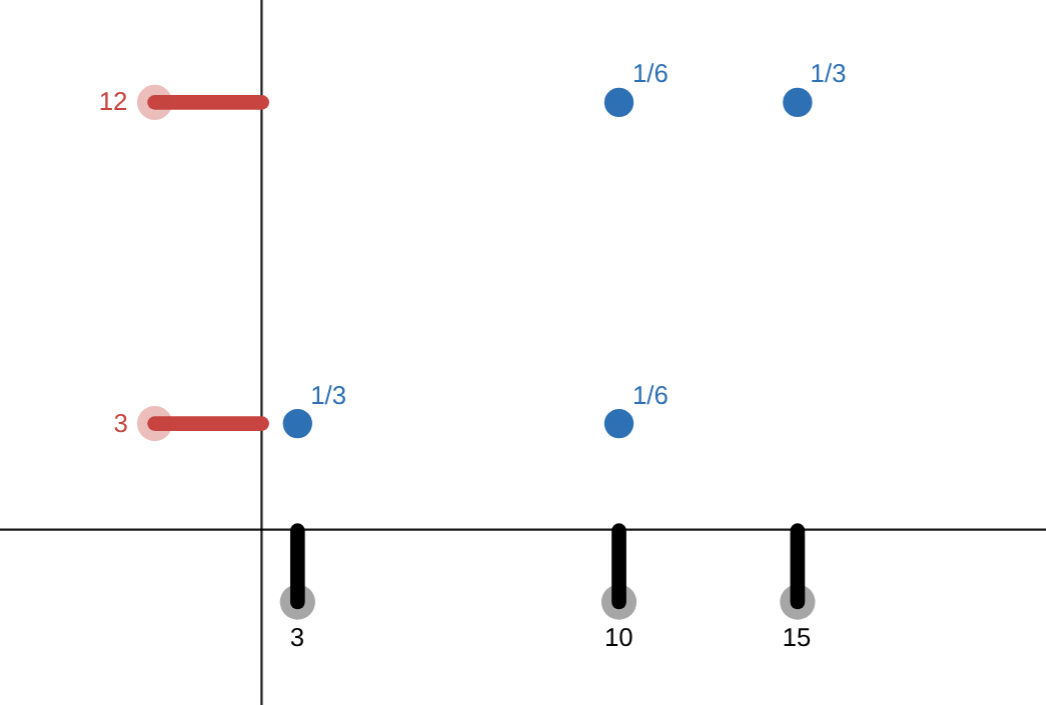
\includegraphics[width=0.5\textwidth]{Picture_2.png}
    \caption{Optimal coupling between two discrete measures.}
    \label{fig:optimal-example}
\end{figure}
Rather than proving the optimality of this linear problem, in Section \ref{section:cm}, we will establish
the condition of $c$-cyclic monotonicity which generalizes the method to solve this discrete problem.

\section{Existence of MKp solution}
The example given above was very simple, but the problem is stated very generally, and it will 
be important to consider general cases, even those where $\mu$ and $\nu$ are neither discrete nor continuous.
To get closer to achieving this goal, we must first prove that the goal is feasible. In other words, we must prove
that there is a coupling that satisfies \eqref{MKp}.

%We need one definition before proceeding

%\begin{definition}[Polish Metric Space]
%    A metric space $(\mathcal{X},d)$ is a Polish space if it contains a countable dense subset and is complete.
%\end{definition}
%All $ \mathbb{R}^{d}$ Euclidean spaces are Polish spaces ($ \mathbb{Q}^{d}$ is a countable dense subset of $ \mathbb{R}^{d}$ for all $d$)
%and so it may prove useful to keep them in mind for the following theorems.


\begin{theorem}[Existence of Optimal Coupling]\label{thm:Existence}
    Let $( \mathbb{R},\mu), ( \mathbb{R},\nu)$ be two probability spaces on $ \mathbb{R}$. Let $c : \mathbb{R}^2 \rightarrow \mathbb{R}^{+} \cup \{+\infty\} $ be an unsigned continuous cost function.
    Then there exists $\pi \in \Pi(\mu,\nu)$ satisfying \eqref{MKp}.
\end{theorem}

\begin{remark}
    In reality this theorem is true even when $ (\mathbb{R}, \mathbb{R})$ are replaced by $(\mathcal{X}, \mathcal{Y})$, which are any separable complete metrizable topological spaces (Polish spaces), and $c$ is only lower semicontinuous and bounded below
    by two lower semicontinuous functions. However, in the interest of time we will focus on this simpler case.
\end{remark}

To prove this theorem in full generality we must use the power of weak convergence covered in Tao's \emph{An Epsilon of Room} \citep{tao2010epsilon}, but luckily with our reduced assumptions we can prove it directly. We will still need
some building blocks.

\begin{definition}[Weak Convergence]
    A sequence of probability measures $(\pi_k)_{k \in \mathbb{N}}$ on $ \mathbb{R}^{d}$ converges weakly to a
    measure $\pi$ on $ \mathbb{R}^{d}$ if for every continuous bounded function $f: \mathbb{R}^d \rightarrow \mathbb{R}$
    \[
    \int_{ \mathbb{R}^d}^{}fd\pi_k \rightarrow \int_{ \mathbb{R}^d}^{}f d\pi
    \] 
    as $k \rightarrow \infty$.
\end{definition}

This definition opens up a way for us to guarantee an optimal coupling via a sequential compactness argument.

\begin{lemma}\label{lemma:lemma_1}
    Let $c: \mathbb{R}^2 \rightarrow \mathbb{R}^{+} \cup \{+\infty\}$. Let $(\pi_k)_{k \in \mathbb{N}}$ be 
    a sequence of probability measures on $ \mathbb{R}^2$ converging weakly
    to some $ \pi$ probability measure on $ \mathbb{R}^2$. Then
    \[
    \int_{ \mathbb{R}^2}^{}c d\pi \le \liminf_{k\to \infty} \int_{ \mathbb{R}^2}^{} c d\pi_k
    \] 
\end{lemma}
\begin{proof}
    Let
    \[
    c_l(x,y) = 
    \begin{cases}
        c(x,y) & c(x,y) \le l\\
        l & c(x,y) > l
    \end{cases}
    \] 
    Then $(c_l)_{l \in \mathbb{N}}$ is a monotone nondecreasing sequence of continuous bounded functions
    and by the monotone convergence theorem
    \[
    \int_{ \mathbb{R}^2}^{}c d\pi = \lim_{l\to \infty} \int_{ \mathbb{R}^2}^{}c_l d\pi
    \] 
    By the definition of weak convergence on our continuous bounded functions we have
    \[
    \int_{ \mathbb{R}^2}^{}c_l d\pi = \lim_{k\to \infty} \int_{ \mathbb{R}^2}^{}c_l d\pi_k
    \] 
    Additionally for all $l$ and monotonicity of $(c_l)_l$
     \[
    \int_{ \mathbb{R}^2}^{}c_l d\pi_k \le \int_{ \mathbb{R}^2}^{}c d\pi_k
    \] 
    Putting this together, we have
    \[
    \int_{ \mathbb{R}^2}^{}c d\pi = \lim_{l\to \infty} \lim_{k\to \infty}\int_{ \mathbb{R}^2}^{}c_l d\pi_k \le \liminf_{k\to \infty}\int_{ \mathbb{R}^2}^{} c d\pi_k
    \] 
\end{proof}

This result is important because if we can construct a sequence of couplings converging weakly to 
another coupling and the infimum of the MKp we can conclude that the limiting coupling is optimal.

\begin{lemma}\label{lemma:tightness}
    Let $\mu, \nu$ be two probability measures on $ \mathbb{R}$. Then for all $\epsilon > 0$,
    there exists $K \subset \mathbb{R}^2$ compact, such that for all $\pi \in \Pi(\mu,\nu)$,
    $\pi( \mathbb{R}^2 \setminus K) < \epsilon$.
\end{lemma}
\begin{proof}
    Fix $\epsilon > 0$.
    By continuity from below of measure we have
    \[
        \lim_{R\to \infty}\mu([-R,R]) = \mu( \mathbb{R}) = 1
    \] 
    There exists $R$ such that 
    \[
        \mu( \mathbb{R} \setminus [-R,R]) < \frac{\epsilon}{2} \qquad \nu( \mathbb{R} \setminus [-R,R]) < \frac{\epsilon}{2}
    \] 
    $K := [-R,R] \times [-R,R]$ is a compact set in  $ \mathbb{R}^2$.
    Note that the complement of this rectangle is contained in the union of the complements of its sides
    \[
        \mathbb{R}^2 \setminus K \subset (( \mathbb{R} \setminus [-R,R]) \times \mathbb{R}) \cup ( \mathbb{R} \times ( \mathbb{R} \setminus [-R,R]))
    \] 
    Let $\pi \in \Pi(\mu,\nu)$ be arbitrary, using marginal properties and subadditivity of measures:
    \begin{align*}
        \pi( \mathbb{R}^2 \setminus K) &\le \pi(\mathbb{R} \setminus [-R,R]) \times \mathbb{R}) + \pi( \mathbb{R} \times ( \mathbb{R} \setminus [-R,R]))\\
                                       &= \mu( \mathbb{R} \setminus [-R,R]) + \nu( \mathbb{R} \setminus [-R,R])\\
                                       &< \frac{\epsilon}{2} + \frac{\epsilon}{2} = \epsilon
    \end{align*}
    Since $\epsilon$ was arbitrary we have proved this lemma.
\end{proof}
\begin{remark}
    This proof is also valid when the sets are Polish spaces.
\end{remark}

Now that we have established tightness of the couplings we can say more about the existence of a limit.
This fundamental result, originally formulated by Yuri Prokhorov in 1956 \citep{prokhorov1956convergence}, shows that under this assumption, a space of measures is relatively compact. 
\begin{theorem}[Prokhorov's Theorem]\label{thm:prokhorov}
    Let $(\pi_k)_{k \in \mathbb{N}}$ be a sequence of probability measures on $\mathbb{R}$. If the sequence is tight (satisfies the condition in Lemma \ref{lemma:tightness}), then there exists a subsequence $(\pi_{k_j})_{j \in \mathbb{N}}$ that converges weakly to some probability measure $\pi$.
\end{theorem}

To prove the existence of a weak limit, we utilize the correspondence between probability measures on $\mathbb{R}^d$ and their cumulative distribution functions (CDFs). 

\begin{lemma}[Helly's Selection Principle]\label{lemma:helly}
    Let $(F_k)_{k \in \mathbb{N}}$ be a sequence of uniformly bounded, non-decreasing functions on $\mathbb{R}$. Then there exists a subsequence $(F_{k_j})$ and a non-decreasing, right-continuous function $F$ such that $F_{k_j}(x) \to F(x)$ pointwise at all continuity points of $F$.
\end{lemma}

\begin{proof}
    Let $S = \{q_1,q_2\dots,\}$ be an enumeration of $ \mathbb{Q}$. Consider the sequence at $q_1$
    $(F_k(q_1))_k$. Since the functions are uniformly bounded this is a bounded sequence of real numbers and
    so there exists a convergent subsequence. Call it $F_{1,k}$. Proceeding in this way inductively
    create a subsequence $F_{n,k}$ of the previous sequence  $F_{n-1,k}$ such that it converges for  $q_n$.
    Then the sequence  $F_{k,k}$ converges for every  $q \in \mathbb{Q}$. Let $G(q) = \lim_{k\to \infty}F_{k,k}(q)$ for all $q \in \mathbb{Q}$.
    Extend $G$ to $F : \mathbb{R} \rightarrow \mathbb{R}$ by letting
    \[
        F(x) = \inf \{G(q) : q \in \mathbb{Q}, q > x \}
    \] 
    First, if $y > x$, then it is easy to see that  $F(y) \ge F(x)$ since the infimum is being taken over a smaller set.
    Additionally, $F$ is right-continuous. Let $(x_n)_n \subset \mathbb{R}$ be a sequence such that $x_1 \ge x_2 \ge \dots$ and $\lim_{i\to \infty}x_i = x$.
    For any $\epsilon > 0$, there exists a rational $q > x$ such that  $G(q) < F(x) + \epsilon$. For sufficiently large $n$,
    we have $x \le x_n < q$ and by monotonicity of  $F$ we have
     \[
    F(x) \le F(x_n) \le G(q) < F(x) + \epsilon
    \] 
    Thus,
    \[
    \lim_{n\to \infty} F(x_n) = F(x)
    \] 
    This proves right-continuity.
    Finally, we must show that $F_{k,k}$ converges to $F$ at every point $x$ where  $F$ is continuous.
    Let $x$ be a continuity point of $F$. For any rational  $q > x$ monotonicity of the $F_k$  implies
    \[
        F_{k,k}(x) \le F_{k,k}(q)
    \] 
    So 
    \[
        \limsup_{k\to \infty}F_{k,k}(x) \le \lim_{k\to \infty}F_{k,k}(q) = G(q)
    \] 
    Taking the infimum over all rational $q > x$, we get
     \[
         \limsup_{k\to \infty}F_{k,k}(x) \le F(x)
    \] 
    Similarly, for all rational $r < x$ we have  $F_{k,k}(r) \le F_{k,k}(x)$ and so we have
     \[
         G(r) \le \liminf_{k\to \infty} F_{k,k}(x)
    \] 
    but since $x$ is a continuity point $\sup\{G(r) : r \in \mathbb{Q}, r \le x\} = F(x)$ by monotonicity of $G$ and that  $G = F$ on  $ \mathbb{Q}$ 
    so we can conclude
    \[
        F(x) \le \liminf_{k\to \infty} F_{k,k}(x)
    \] 
    Taking these two facts together, we get
    \[
        \lim_{k\to \infty}F_{k,k}(x) = F(x)
    \] 
    for all $x$ that are continuity points of $F$.
\end{proof}
\begin{remark}[Extension to $\mathbb{R}^d$]
    The proof of Lemma \ref{lemma:helly} relies on the countability of the dense subset $\mathbb{Q} \subset \mathbb{R}$.
    Since $\mathbb{Q}^d$ is also a countable dense subset of $\mathbb{R}^d$,
    the same diagonalization argument allows us to extract a subsequence of CDFs $F_{k_j}(x_1, \dots, x_d)$
    that converges at every continuity point. Consequently, Helly's Selection Principle holds for $\mathbb{R}^d$.
    A rigorous proof can be found in Theorem 11.1.1 of \citet{dudley2002real}.
\end{remark}

With this tool, we can prove Prokhorov's Theorem.

\begin{proof}[Proof of Theorem~\ref{thm:prokhorov}]
    Let $F_k$ be the CDF corresponding to $\mu_k$, that is $F_k(x) = \mu_k(\{y \in \mathbb{R}, y \le x\})$. Since $\mu_k$ are probability measures $0 \le F_k(x) \le 1$ so the sequence is uniformly bounded. Note that $F_k$ satisfies the conditions of Helly's Selection Principle \ref{lemma:helly}.

    By Helly's Selection Principle (Lemma \ref{lemma:helly}), there exists a subsequence (which we still denote as $F_k$) and a non-decreasing right-continuous function $F$ such that $F_k \to F$ at continuity points.
    We must show that $F$ is the CDF of a valid probability measure. Recall the moving bump example provided in lecture; we do not want our sequence to lose mass in the limit.
    Fix $\epsilon > 0$. Since the sequence is tight, there exists a compact interval $K = [-M, M]$ such that for all $k$, $\mu_k(K^c) < \epsilon$.
    In terms of our CDFs, this says that for all  $k$  $F_k(M) - F_k(- M) \ge 1 - \epsilon$.
    In particular, for all continuity points  $|x| > M$  $F(x) - F(-x) \ge 1 -\epsilon$
    Sending $\epsilon$ to $0$ and picking larger  $M$'s,
    we see that
     \[
    \lim_{x \to \infty} F(x) - F(-x) = 1 \;\;\; \lim_{x\to \infty}F(x) = 1 \;\;\;\; \lim_{x\to -\infty}F(x) = 0
    \] 
    Thus $F$ is a CDF.
    Additionally, corresponding to this CDF, there exists a unique Borel probability measure $\mu$, the Lebesgue-Stieltjes measure, satisfying $\mu([a,b]) = F_+(b) - F_-(a)$ as outlined in Theorem 1.7.9 of Tao \citep{Tao2011Measure}.
    The fact that $\mu_k$ converges weakly to $\mu$ is unfortunately involved, but can be found in Theorems 3.2.8 and 3.2.9 of Durrett's Probability \citep{Durrett2019}.
\end{proof}
\begin{remark}
    As with \ref{lemma:helly}, this Theorem is true in the general setting of Polish spaces,
    see Theorem 5.1 \citet{billingsley1999convergence} for exact details.
\end{remark}

Despite my efforts to build this theory using only the tools taught in \citep{Tao2011Measure} I will introduce one theorem that will be useful in the next lemma.
The Pi-Lambda theorem, attributed to Eugene Dynkin, allows statements that are true on a "basic set" to be expanded to the $\sigma$-algebra completion of the set.
\begin{theorem}[Pi-Lambda Theorem]\label{thm:pilambda}
    A set $\mathcal{P} \subset 2^{\Omega}$ is a $\pi$-system if
    \begin{enumerate}
        \item $\mathcal{P}$ is non-empty
        \item $A, B \in \mathcal{P} \implies A \cap B \in \mathcal{P}$
    \end{enumerate}
    A set $\mathcal{L} \subset 2^{\Omega}$ is a $\lambda$-system if
    \begin{enumerate}
        \item  $\emptyset \in \mathcal{L}$
        \item $A \in \mathcal{L} \implies \Omega \setminus A \in \mathcal{L}$
        \item if $A_1,A_2,\dots$ are a sequence of pairwise disjoint sets in $\mathcal{L}$ then
            $\bigcup_{i=1}^{\infty}A_i \in \mathcal{L}$
    \end{enumerate}
    If $\mathcal{P}$ is a  $\pi$-system and $\mathcal{L}$ is a  $\lambda$-system and $\mathcal{P} \subset \mathcal{L}$ then $\sigma(\mathcal{P}) \subset \mathcal{L}$
\end{theorem}
A proof can be found in Theorem A.1.4 of \citet{Durrett2019}.

\begin{lemma}\label{lemma:limit_coupling}
    Let $(\pi_k)_k$ be a sequence of couplings in $\Pi(\mu,\nu)$ for some probability measures $\mu,\nu$ on $ \mathbb{R}$.
    Suppose further that $\pi_k$ converges weakly to $\pi$, a measure on $ \mathbb{R}^2$; then $\pi \in \Pi( \mu, \nu)$.
\end{lemma}
\begin{proof}
    We wish to show that the marginals of $\pi$ are exactly $\mu$ and $\nu$.
    Let $\phi \in C_b( \mathbb{R})$ be a continuous bounded function on $ \mathbb{R}$.
    By the definition of the marginal
    \[
    \int_{ \mathbb{R}^2}^{} \phi(x) d\pi(x,y) =  \int_{ \mathbb{R}}^{}\phi(x) d\pi_1(x)
    \] 
    where $\pi_1$ is the first marginal of $\pi$.
    But we also have
    \[
    \int_{ \mathbb{R}^2}^{}\phi(x)d\pi(x,y) = \lim_{k\to \infty} \int_{ \mathbb{R}^2}^{}\phi(x)d\pi_k(x,y) = \int_{ \mathbb{R}}^{}\phi(x)d\mu(x)
    \] 
    by definition of weak convergence.
    So, we can conclude that for all continuous bounded functions $\phi$
    \[
    \int_{ \mathbb{R}}^{}\phi(x)d\pi_1(x) = \int_{ \mathbb{R}}^{}\phi(x) d\mu(x).
    \] 
    Let $F$ be any closed set and define
    \[
    g_l(x) = \max(0,1 - ld(x,F))
    \] 
    where $d(x,F) = \inf\{d(x,y) : y \in F\}$. \\
    Then $g_l(x) \ge 1_{F}(x)$ and is continuous, with $\lim_{l\to \infty}g_l(x) = 1_{F}(x)$. By the dominated convergence theorem, since $|g_l| \le 1$ and is thus absolutely integrable with respect to every probability measure, we have:
    \[
    \pi_1(F) = \int_{ \mathbb{R}}^{} 1_F(x) d\pi_1(x) = \lim_{l\to \infty} \int_{ \mathbb{R}}^{}g_l(x) d\pi_1(x) = \lim_{l\to \infty} \int_{ \mathbb{R}}^{}g_l(x) d\mu(x)  = \int_{ \mathbb{R}}^{}1_F(x) d\mu(x) = \mu(F)
    \] 
    So $\pi_1$ and $\mu$ agree on all closed sets.
    Let $ \mathcal{P}$ be the set of all closed sets.
    Let $\mathcal{S} \subset \mathcal{B}( \mathbb{R})$ be the collection of Borel sets on $ \mathbb{R}$ such that $A \in \mathcal{S} \implies \mu(A) = \pi_1(A)$.
    Then $\mathcal{S}$ contains all closed sets on  $ \mathbb{R}$ and
    \begin{align*}
        \mathbb{R} \in S \;\;\;\;\;\;\;\;&\text{since $ \mathbb{R}$ is closed}\\
        A \in S \implies& \pi_1(A^{c}) = 1 - \pi_1(A) = 1 - \mu(A) = \mu(A^{c})\\
        A_1, A_2, \dots, \in S, A_i \cap A_j = \emptyset, \forall i \ne j \implies& \pi_1 \left( \bigcup_{i=1}^{\infty}A_i \right) = \sum_{i=1}^{\infty}\pi_1(A_i) = \sum_{i=1}^{\infty}\mu(A_i) = \mu\left(\bigcup_{i=1}^{\infty}A_i\right)
    \end{align*}
    Thus $\mathcal{S}$ is a  $\lambda$-system. Since the set of closed sets is closed under finite intersections, it is a $\pi$-system.
    By the $\pi-\lambda$ theorem \ref{thm:pilambda}, $\sigma( \mathcal{P}) \subset \mathcal{S}$ but $\sigma(\mathcal{P}) = \mathcal{B}( \mathbb{R})$. We can conclude that
    $\pi_1(A) = \mu(A)$ for all Borel sets $A$ on  $ \mathbb{R}$. Thus $\pi_1 = \mu$ and $\pi$ admits $\mu$ as its first marginal.\\
    The argument for the other direction is equivalent and we conclude that $\pi \in \Pi(\mu, \nu)$ whenever it is the weak limit of couplings in $\Pi(\mu,\nu)$.
\end{proof}

We have now shown that our space of couplings $\Pi(\mu,\nu)$ is sequentially compact with respect
to weak convergence. We have also shown that when a sequence of couplings $(\pi_k)_k$ converges weakly to $\pi$ our transport cost cannot increase in the limit.
Putting these together we can finally argue the existence of an optimal transport plan:


\begin{proof}[Proof of Theorem~\ref{thm:Existence}]
    Fix $\mu,\nu$ probability spaces on $ \mathbb{R}$ and $c : \mathbb{R}^2 \rightarrow \mathbb{R}^{+} \cup \{+ \infty\}$ unsigned continuous cost function.
    Then, by Lemma~\ref{lemma:tightness}, $\Pi(\mu,\nu)$ is tight. Let $(\pi_k)_{k \in \mathbb{N}}$ be a sequence of couplings such that
    \[
        \lim_{k\to \infty} \int_{ \mathbb{R}^2}^{}c(x,y)d\pi_k(x,y) = \inf_{\pi \in \Pi(\mu,\nu)} \int_{ \mathbb{R}^2}^{}c(x,y) d\pi(x,y)
    \] 
    Then, by Prokhorov's Theorem~\ref{thm:prokhorov}, there exists a subsequence $(\pi_{k_j})_{j \in \mathbb{N}}$ converging to some probability measure $\pi$ weakly.
    By Lemma~\ref{lemma:limit_coupling} we know $\pi \in \Pi(\mu,\nu)$ and by Lemma~\ref{lemma:lemma_1}
    \[
        \int_{ \mathbb{R}^2}^{}c(x,y)d\pi(x,y) \le \liminf_{j\to \infty} \int_{ \mathbb{R}^2}^{}c(x,y)d\pi_{k_j}(x,y) = \inf_{\eta \in \Pi(\mu,\nu)} \int_{ \mathbb{R}^2}^{}c(x,y) d\eta(x,y)
    \] 
    And so $\pi$ is an optimal transport plan.
\end{proof}

\subsection{Counterexample}
To illustrate why we need the above conditions to guarantee the existence of an optimal coupling, consider the following counterexample.
Consider the space $ \mathcal{X} = \mathcal{Y} = [0,1]$ equipped with the Lebesgue measure $\mu = \nu = \lambda|_{[0,1]}$.
Define the cost function
\[
c(x,y) :=
\begin{cases}
    2 & x = y\\
    |x-y| & x \neq y.
\end{cases}
\] 
Then clearly $c$ is continuous everywhere except at all points where $x = y$.
Consider the sequence of transport maps  $T_n(x) = (x + \frac{1}{n}) \pmod 1$ where $\pi_n = (\mathrm{Id}, T_n)_*(\mu) $ the pushforward measure.
Then the couplings $\pi_n$ are supported on the lines $y = (x + \frac{1}{n}) \pmod 1$ and as $n \to \infty$
the $\pi_n$ converge to $\pi_{id} = (\mathrm{Id},\mathrm{Id})_*(\mu)$. Additionally
\[
\lim_{n\to \infty} \int_{}^{}c(x,y) d\pi_n(x,y) = \lim_{n\to \infty} \int_{}^{} c(x, T_n(x)) d \mu(x) = \lim_{n\to \infty} \frac{1}{n} = 0.
\] 
However
\[
    \int_{}^{}c(x,y) d \pi_{id}(x,y) = \int_{0}^{1} c(x,x) dx = \int_{0}^{1} 2 dx = 2.
\] 
We can see that the infimum cost must be 0, since our cost function is strictly positive and there exists a sequence of couplings approaching this value.
The infimum is unable to be attained since any coupling $\pi$ with
\[
\int_{}^{}c(x,y) d\pi(x,y) = 0
\] 
would mean that $c(x,y) = 0$  $\pi$-almost everywhere. However there is no point $(x,y)$ on  $[0,1] \times [0,1]$ where the cost is zero, so this can never be the case.
Thus the optimal coupling is not achievable. From this we can see why one of our conditions of continuity (more exactly, lower semicontinuity) is necessary to guarantee an optimal coupling.


\section{Characterizing Optimality: $c$-Cyclic Monotonicity}\label{section:cm}
Now that we are guaranteed an optimal solution, let's see what we can say about the nature of optimal couplings.

\begin{definition}[c-Cyclic Monotonicity \citep{villani2008ot}]
    Let $ \mathcal{X}, \mathcal{Y}$ be sets and $c : \mathcal{X} \times \mathcal{Y} \rightarrow (-\infty, \infty]$ be a function.
    A subset $A \subset \mathcal{X} \times \mathcal{Y}$ is $c$-cyclically monotone if, for
    any $N \in \mathbb{N}$, and any collection $(x_1,y_1), \dots, (x_N, y_N)$ of points in $A$
     \[
         \sum_{i=1}^{N}c(x_i,y_i) \le \sum_{i=1}^{N}c(x_i,y_{i+1})
    \] 
    with $y_{N+1} = y_1$. A coupling is said to be $c$-cyclically monotone if it is supported on a $c$-cyclically monotone set.
\end{definition}

Intuitively, our optimal coupling should be $c$-cyclically monotone since if it were not the case we can "shuffle mass around" to reduce our total cost.

\begin{proposition}[$c$-Cyclic Monotonicity if and only if Optimality]\label{cciffo}
    Let $\mu, \nu \in P( \mathbb{R})$ be discrete measures (i.e.  $\mu = \sum_{i=1}^{n}p_i \delta_{x_i}, \nu = \sum_{i=1}^{m}q_i \delta_{y_i}$)
    and let $c : \mathbb{R}^2 \rightarrow \mathbb{R} \cup \{+\infty\}$ be a continuous cost function. 
    A coupling $\pi \in \Pi(\mu,\nu)$ is optimal if and only if it is $c$-cyclically monotone.
\end{proposition}
I will split this proof into its two parts.
\begin{proof}[Proof of $\Rightarrow$ direction]
    Let $\pi \in \Pi(\mu,\nu)$ be optimal. Assume for contradiction that it is not supported
    on a $c$-cyclically monotone set. Then there exists a set of points $A = \{(x_{j_1},y_{j_1}),\dots,(x_{j_k},y_{j_k})\}$ such that
    $\pi(x_{j_l},y_{j_l}) > \epsilon > 0$ for each $l$, and
    \[
        \sum_{l=1}^{k}c(x_{j_l},y_{j_{l+1}}) < \sum_{l=1}^{k}c(x_{j_l},y_{j_l})
    \] 
    Then construct $\tilde \pi$ by adjusting $\pi $ along this cycle. 
    \begin{enumerate}
        \item First, we remove the extra mass from each pair.
            \[
                \tilde \pi(x_{j_l},y_{j_l}) = \pi(x_{j_l},y_{j_l}) - \epsilon
            \] 
        \item We then add that mass to the new pair.
            \[
                \tilde \pi(x_{j_l}, y_{j_{l+1}}) = \pi(x_{j_l}, y_{j_{l+1}}) + \epsilon
            \] 
        \item Keep $\tilde \pi = \pi$ for all other pairs.
    \end{enumerate}
    We must check that $\tilde \pi \in \Pi(\mu,\nu)$. First, all entries remain nonnegative by our choice of $\epsilon$.
    Additionally $\tilde \pi$ is a probability measure since for each point that is weighted $\epsilon$ less, there is another point weighted $\epsilon$ more,
    ensuring the total mass is constant.
    Fix $x_t$ on the support of  $\mu$ then 
    \[
        \tilde \pi (\{x_t\} \times \mathbb{R}) = \sum_{i=1}^{m} \tilde \pi(x_t,y_i) = \sum_{i=1}^{m} \pi(x_t,y_i) = \pi(\{x_t\} \times \mathbb{R}) = \mu(\{x_t\})
    \] 
    This holds because in the sums, for every term where an $\epsilon$ is subtracted, an $\epsilon$ is added to a different term. 
    The same result holds for the second projections, so we can conclude that $\tilde \pi \in \Pi(\mu,\nu)$. Finally,
    we compute
    \begin{align*}
        \int_{ \mathbb{R}^2}^{}c(x,y)d\tilde \pi(x,y) - \int_{ \mathbb{R}^2}^{}c(x,y) d \pi(x,y) &=
        \epsilon \sum_{l=1}^{k}c(x_{j_l},y_{j_{l+1}}) - \epsilon \sum_{l=1}^{k}c(x_{j_l},y_{j_l}) < 0\\ 
    \end{align*}
    holds by our assumption. Thus, the cost of coupling $\tilde \pi$ is less than that of $\pi$, a contradiction.
    Therefore, every optimal coupling is $c$-cyclically monotone.
\end{proof}
\begin{proof}[Proof of $\Leftarrow$ ]
    Let $\pi \in \Pi(\mu,\nu)$ be $c$-cyclically monotone. I wish to show that for any other $\tilde \pi \in \Pi(\mu,\nu)$ 
    $ \pi$ admits a lower cost. First, let's write our couplings in matrix form
    \[
    M(\pi) = 
    \begin{pmatrix} s_{1,1} & \dots & s_{1,m} \\ \vdots & \ddots & \vdots \\ s_{n,1} & \dots & s_{n,m} \end{pmatrix} 
    \qquad 
    M(\tilde \pi) =
    \begin{pmatrix} \tilde s_{1,1} & \dots & \tilde s_{1,m} \\ \vdots & \ddots & \vdots \\ \tilde s_{n,1} & \dots & \tilde s_{n,m} \end{pmatrix} 
    \] 
    where $ \pi(x_i,y_j) = s_{i,j}, \tilde \pi(x_i,y_j) = \tilde s_{i,j}$, $ \sum_{j=1}^{m}s_{i,j} = p_i = \sum_{j=1}^{m}\tilde s_{i,j}$, and $   \sum _{i=1}^{n}s_{i,j} = q_j = \sum_{i=1}^{n}\tilde s_{i,j} $.
    Then, consider the matrix $M(\tilde \pi) - M(\pi)$, an $n \times m$ matrix whose rows and columns sum to 0.
    I claim that $M(\tilde \pi) - M(\pi) = \sum_{l=1}^{L}\alpha_lD_l$ where each $D_l$ 
    is a matrix supported on an even number of indices  $(i_1,j_1), (i_1,j_2),(i_2,j_2),\dots,(i_r,j_1)$, such that
    the first term is negative, then positive, and so on alternating. 
    To show that this is possible, consider a bipartite directed graph with left nodes $(x_1,x_2,\dots,x_n)$ and right nodes $(y_1,y_2,\dots,y_m)$. Let the edge between
    any two nodes $x_i,y_j$ have weight  $\tilde s_{i,j} - s_{i,j}$. Then every node has zero net flow. If every edge has zero weight, we are done; if not, choose an entry  $(i_1,j_1)$ such that
    $\tilde s_{i_1,j_1} - s_{i_1,j_1} < 0$ (a point $x_{i_1},y_{j_1}$ that $\pi$ weights more than $\tilde \pi$). Since the rows sum to zero, there exists an index $j_2$ such that $s_{i_1,j_2} - \tilde s_{i_1,j_2} > 0$. Continuing inductively,
    we can construct an alternating sequence $(i_1,j_1),(i_1,j_2),(i_2,j_2),\dots$
    Since there are only finitely many indices, we must eventually visit one index twice, producing a closed alternating cycle. In this cycle, one term $|\tilde s_{i,j} - s_{i,j}|$ must be the smallest but nonzero. 
    Let $\epsilon$ be this value and construct the matrix $D^{1}_{i_1,j_1} = -\epsilon, D^{1}_{i_1,j_2} = \epsilon, \dots$ and zero everywhere else.
    Then $\sum_{i=1}^{n}D^{1}_{i,j} = 0$ since every index $j$ comes in pairs of opposite signed points which cancel out the sum. The same holds for sums over columns and we see that the matrix $D^{1}$ obeys the same property as $M(\tilde \pi) - M(\pi)$.
    Continuing inductively in this way, we generate a sequence of $D^{1},D^{2},\dots$ of finitely many cycle matrices which sum to $M(\tilde \pi) - M(\pi)$. To see that this process ends in finite time, note that in each stage, at least one index turns to zero in the remaining matrix.
    If we let the cost matrix $C \in \mathbb{R}^{n\times m}$ be such that $C_{i,j} = c(x_i,y_j),$ we can see that 
    \[
    \int_{}^{}c(x,y) d \tilde \pi(x,y) - \int_{}^{}c(x,y) d \pi(x,y) = \langle M(\tilde \pi) - M(\pi), C \rangle_F = \sum_{l=1}^{L} \langle D_l, C \rangle_F
    \] 
    If I can show that $\langle D_l, C \rangle_F \ge 0$ for each $l$, I am done. But
    \[
        \langle D_1, C \rangle_F = \epsilon_l\left( \sum_{}^{} (\text{cost of positive entries of $D^1$}) - \sum_{}^{}(\text{cost of negative entries in $D^{1}$ })\right)
    \] 
    However, the negative points are all areas of the support of $\pi$ of the form $(i_1,j_{1}),(i_2,j_{2}),\dots$ and each positive term is $(i_1,j_{1+1}),(i_2,j_{2+1}),\dots$ and we have
    \[
        \sum_{p=1}^{N}c(x_{i_p},y_{i_p}) \le \sum_{p=1}^{N}c(x_i,y_{i_{p+1}})
    \] 
    So, we conclude
    \[
    \langle D_1, C \rangle_F \ge 0
    \] 
    This further implies that $\tilde \pi$ is not more optimal than $\pi$. Since $\tilde \pi$ was arbitrary, we have that $\pi$ is the optimal solution.
\end{proof}

\begin{remark}
A natural extension of this paper would be to explore other ways of finding optimal solutions including solving the dual problem as proposed by  \citet{kantorovich1942english}.
We now have a strong understanding of why optimal couplings exist and their behavior under certain assumptions. I am encouraged to learn more and keep exploring this fascinating subject in the future.
\end{remark}


\section*{Acknowledgments}
I would like to acknowledge Elias Manuelides for helping me with this project. He inspired me to choose the topic of optimal transport and gave helpful feedback on
an initial draft of this paper.

\bibliographystyle{plainnat}
\bibliography{ot}


\end{document}
